% Options for packages loaded elsewhere
% Options for packages loaded elsewhere
\PassOptionsToPackage{unicode}{hyperref}
\PassOptionsToPackage{hyphens}{url}
%
\documentclass[
  english,
  russian,
  12pt,
  a4paper,
  DIV=11,
  numbers=noendperiod]{scrreprt}
\usepackage{xcolor}
\usepackage{amsmath,amssymb}
\setcounter{secnumdepth}{5}
\usepackage{iftex}
\ifPDFTeX
  \usepackage[T1]{fontenc}
  \usepackage[utf8]{inputenc}
  \usepackage{textcomp} % provide euro and other symbols
\else % if luatex or xetex
  \usepackage{unicode-math} % this also loads fontspec
  \defaultfontfeatures{Scale=MatchLowercase}
  \defaultfontfeatures[\rmfamily]{Ligatures=TeX,Scale=1}
\fi
\usepackage{lmodern}
\ifPDFTeX\else
  % xetex/luatex font selection
\fi
% Use upquote if available, for straight quotes in verbatim environments
\IfFileExists{upquote.sty}{\usepackage{upquote}}{}
\IfFileExists{microtype.sty}{% use microtype if available
  \usepackage[]{microtype}
  \UseMicrotypeSet[protrusion]{basicmath} % disable protrusion for tt fonts
}{}
\usepackage{setspace}
% Make \paragraph and \subparagraph free-standing
\makeatletter
\ifx\paragraph\undefined\else
  \let\oldparagraph\paragraph
  \renewcommand{\paragraph}{
    \@ifstar
      \xxxParagraphStar
      \xxxParagraphNoStar
  }
  \newcommand{\xxxParagraphStar}[1]{\oldparagraph*{#1}\mbox{}}
  \newcommand{\xxxParagraphNoStar}[1]{\oldparagraph{#1}\mbox{}}
\fi
\ifx\subparagraph\undefined\else
  \let\oldsubparagraph\subparagraph
  \renewcommand{\subparagraph}{
    \@ifstar
      \xxxSubParagraphStar
      \xxxSubParagraphNoStar
  }
  \newcommand{\xxxSubParagraphStar}[1]{\oldsubparagraph*{#1}\mbox{}}
  \newcommand{\xxxSubParagraphNoStar}[1]{\oldsubparagraph{#1}\mbox{}}
\fi
\makeatother


\usepackage{longtable,booktabs,array}
\usepackage{calc} % for calculating minipage widths
% Correct order of tables after \paragraph or \subparagraph
\usepackage{etoolbox}
\makeatletter
\patchcmd\longtable{\par}{\if@noskipsec\mbox{}\fi\par}{}{}
\makeatother
% Allow footnotes in longtable head/foot
\IfFileExists{footnotehyper.sty}{\usepackage{footnotehyper}}{\usepackage{footnote}}
\makesavenoteenv{longtable}
\usepackage{graphicx}
\makeatletter
\newsavebox\pandoc@box
\newcommand*\pandocbounded[1]{% scales image to fit in text height/width
  \sbox\pandoc@box{#1}%
  \Gscale@div\@tempa{\textheight}{\dimexpr\ht\pandoc@box+\dp\pandoc@box\relax}%
  \Gscale@div\@tempb{\linewidth}{\wd\pandoc@box}%
  \ifdim\@tempb\p@<\@tempa\p@\let\@tempa\@tempb\fi% select the smaller of both
  \ifdim\@tempa\p@<\p@\scalebox{\@tempa}{\usebox\pandoc@box}%
  \else\usebox{\pandoc@box}%
  \fi%
}
% Set default figure placement to htbp
\def\fps@figure{htbp}
\makeatother



\ifLuaTeX
\usepackage[bidi=basic,provide=*]{babel}
\else
\usepackage[bidi=default,provide=*]{babel}
\fi
% get rid of language-specific shorthands (see #6817):
\let\LanguageShortHands\languageshorthands
\def\languageshorthands#1{}


\setlength{\emergencystretch}{3em} % prevent overfull lines

\providecommand{\tightlist}{%
  \setlength{\itemsep}{0pt}\setlength{\parskip}{0pt}}



 
\usepackage[backend=biber,langhook=extras,autolang=other*]{biblatex}
\addbibresource{bib/cite.bib}

\usepackage[]{csquotes}

\KOMAoption{captions}{tableheading}
\usepackage{indentfirst}
\usepackage{float}
\floatplacement{figure}{H}
\usepackage{libertine}
\makeatletter
\@ifpackageloaded{caption}{}{\usepackage{caption}}
\AtBeginDocument{%
\ifdefined\contentsname
  \renewcommand*\contentsname{Содержание}
\else
  \newcommand\contentsname{Содержание}
\fi
\ifdefined\listfigurename
  \renewcommand*\listfigurename{Список иллюстраций}
\else
  \newcommand\listfigurename{Список иллюстраций}
\fi
\ifdefined\listtablename
  \renewcommand*\listtablename{Список таблиц}
\else
  \newcommand\listtablename{Список таблиц}
\fi
\ifdefined\figurename
  \renewcommand*\figurename{Рисунок}
\else
  \newcommand\figurename{Рисунок}
\fi
\ifdefined\tablename
  \renewcommand*\tablename{Таблица}
\else
  \newcommand\tablename{Таблица}
\fi
}
\@ifpackageloaded{float}{}{\usepackage{float}}
\floatstyle{ruled}
\@ifundefined{c@chapter}{\newfloat{codelisting}{h}{lop}}{\newfloat{codelisting}{h}{lop}[chapter]}
\floatname{codelisting}{Список}
\newcommand*\listoflistings{\listof{codelisting}{Листинги}}
\makeatother
\makeatletter
\makeatother
\makeatletter
\@ifpackageloaded{caption}{}{\usepackage{caption}}
\@ifpackageloaded{subcaption}{}{\usepackage{subcaption}}
\makeatother
\usepackage{bookmark}
\IfFileExists{xurl.sty}{\usepackage{xurl}}{} % add URL line breaks if available
\urlstyle{same}
\hypersetup{
  pdftitle={Отчет по лабораторной работе №3},
  pdfauthor={Габдуллина Александра Булатовна},
  pdflang={ru-RU},
  hidelinks,
  pdfcreator={LaTeX via pandoc}}


\title{Отчет по лабораторной работе №3}
\usepackage{etoolbox}
\makeatletter
\providecommand{\subtitle}[1]{% add subtitle to \maketitle
  \apptocmd{\@title}{\par {\large #1 \par}}{}{}
}
\makeatother
\subtitle{Простейший вариант}
\author{Габдуллина Александра Булатовна}
\date{}
\begin{document}
\maketitle

\renewcommand*\contentsname{Содержание}
{
\setcounter{tocdepth}{1}
\tableofcontents
}
\listoffigures
\listoftables

\setstretch{1.5}
\chapter{Цель
работы}\label{ux446ux435ux43bux44c-ux440ux430ux431ux43eux442ux44b}

Целью работы является освоение процедуры оформления отчетов с помощью
легковесного языка разметки Markdown.

\chapter{Задание}\label{ux437ux430ux434ux430ux43dux438ux435}

\begin{enumerate}
\def\labelenumi{\arabic{enumi}.}
\tightlist
\item
  В соответствующем каталоге сделайте отчёт по лабораторной работе № 2 в
  формате Markdown. В качестве отчёта необходимо предоставить отчёты в
  трех форматах: pdf, docx и md.
\item
  Загрузите файлы на github.
\end{enumerate}

\chapter{Выполнение лабораторной
работы}\label{ux432ux44bux43fux43eux43bux43dux435ux43dux438ux435-ux43bux430ux431ux43eux440ux430ux442ux43eux440ux43dux43eux439-ux440ux430ux431ux43eux442ux44b}

3.4. Переходим в нужный репозиторий (с помощью команды cd) и выгружаем
данные с гитхаба (git pull). (рис1)

\begin{figure}

{\centering 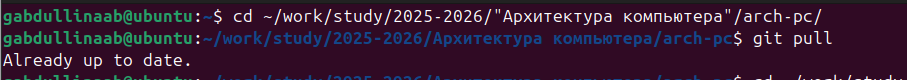
\includegraphics[width=0.9\linewidth,height=\textheight,keepaspectratio]{image/рис1.png}

}

\caption{рис1}

\end{figure}%

С помощью make создаем файлы report.pdf и report.docx (рис2). Проверяем,
создались ли файлы в директории (рис3).

\begin{figure}

{\centering 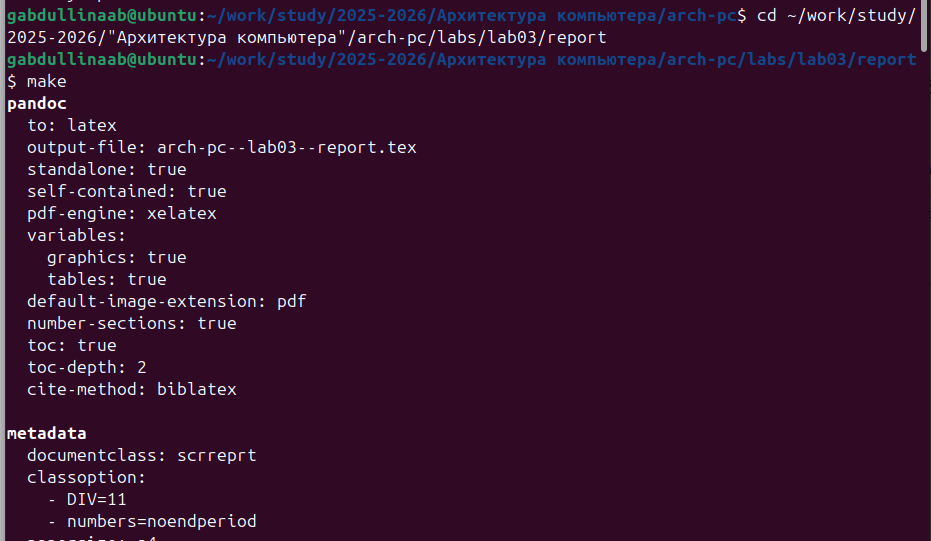
\includegraphics[width=0.9\linewidth,height=\textheight,keepaspectratio]{image/рис2.png}

}

\caption{рис2}

\end{figure}%

\begin{figure}

{\centering 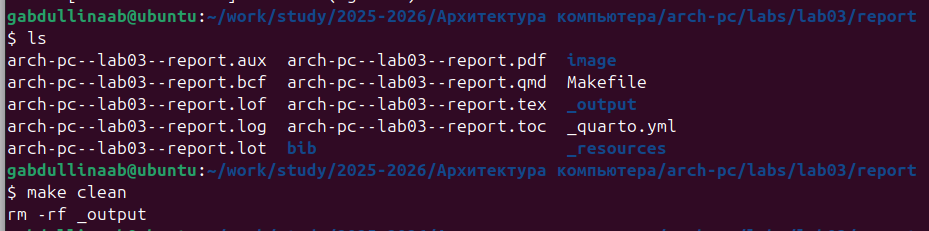
\includegraphics[width=0.9\linewidth,height=\textheight,keepaspectratio]{image/рис3.png}

}

\caption{рис3}

\end{figure}%

С помощью команды make clean удаляем созданные ранее файлы (рис4).
Проверяем, удалились ли они в файлах (рис5 - нет папки \_output -- файлы
удалились)

\begin{figure}

{\centering 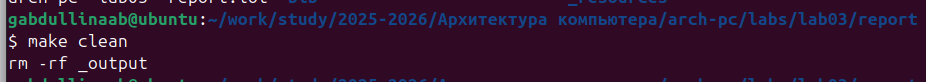
\includegraphics[width=0.9\linewidth,height=\textheight,keepaspectratio]{image/рис4.png}

}

\caption{рис4}

\end{figure}%

\begin{figure}

{\centering 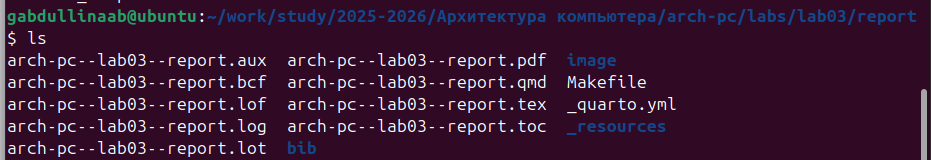
\includegraphics[width=0.9\linewidth,height=\textheight,keepaspectratio]{image/рис5.png}

}

\caption{рис5}

\end{figure}%

Копируем файл report.qmd из папки с шаблонами, т.к. при выполнении
лабораторной работы 2 файлы report создались не совсем корректно - они
имеют название \enquote{arch-pc--lab03--report.qmd} и
arch-pc--lab03pparch-pc--lab03--report.qmd''. Их почему-то создалось 2 и
их названия некорректны. Их можно было бы переименовать или оставить
такими, как есть, ибо команда make создает pdf и docx файлы и для них,
но я решил, что лучше скопировать оригинальный файл из шаблонов (папка
templates) (рис6)

\begin{figure}

{\centering 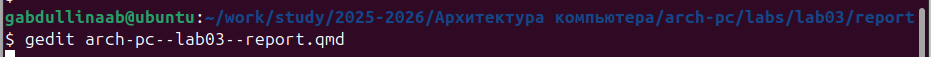
\includegraphics[width=0.9\linewidth,height=\textheight,keepaspectratio]{image/рис6.png}

}

\caption{рис6}

\end{figure}%

С помощью gedit открываем файл report.qmd (рис7)

\begin{figure}

{\centering 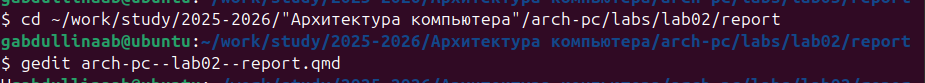
\includegraphics[width=0.9\linewidth,height=\textheight,keepaspectratio]{image/рис7.png}

}

\caption{рис7}

\end{figure}%

Изучаем файл и редактируем его согласно инструкциям.

3.5. Переходим в каталог лабораторной работы 2 с помощью cd, открываем
файл отчета с помощью gedit.(рис8)

\begin{figure}

{\centering 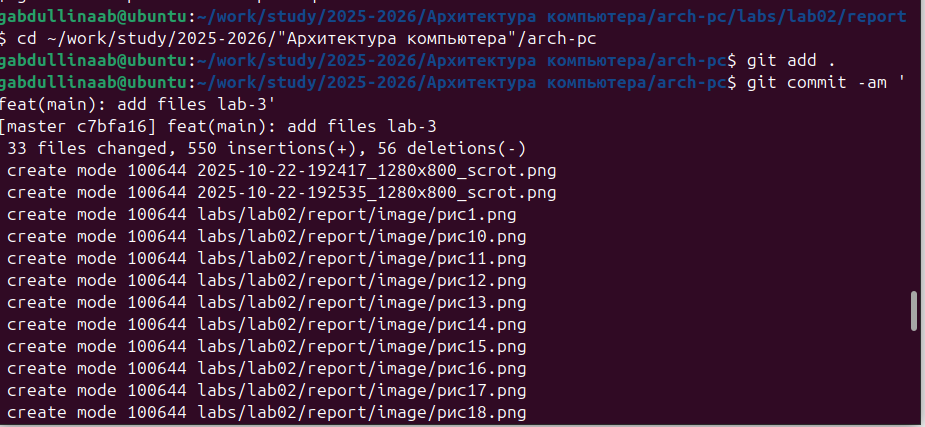
\includegraphics[width=0.9\linewidth,height=\textheight,keepaspectratio]{image/рис8.png}

}

\caption{рис8}

\end{figure}%

Редактируем отчет (рис9).

\begin{figure}

{\centering 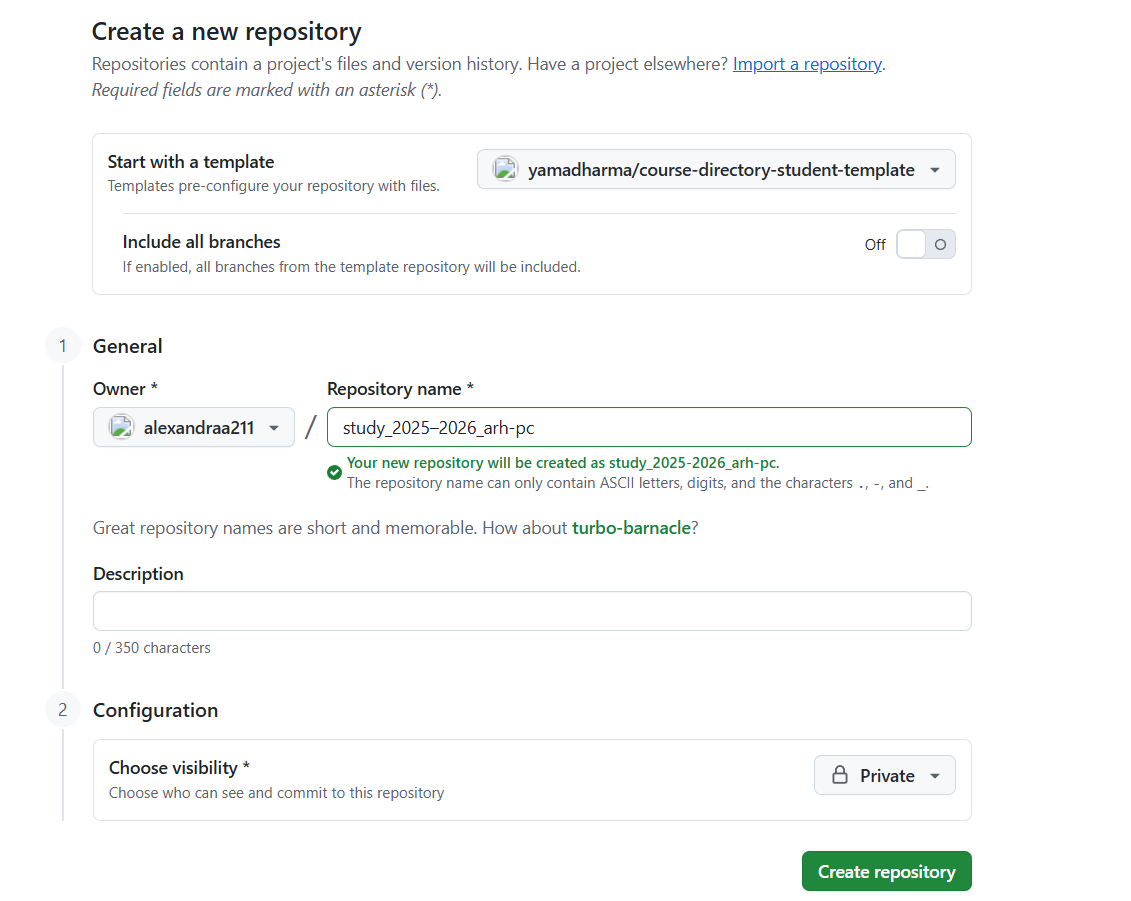
\includegraphics[width=0.9\linewidth,height=\textheight,keepaspectratio]{image/рис9.png}

}

\caption{рис9}

\end{figure}%

Формируем отчет с помощью make (рис10).

\begin{figure}

{\centering 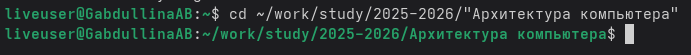
\includegraphics[width=0.9\linewidth,height=\textheight,keepaspectratio]{image/рис10.png}

}

\caption{рис10}

\end{figure}%

Отправляем отчет на github (рис11,рис12).

\begin{figure}

{\centering 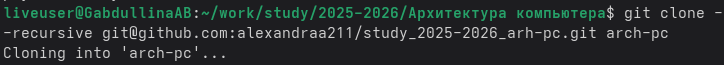
\includegraphics[width=0.9\linewidth,height=\textheight,keepaspectratio]{image/рис11.png}

}

\caption{рис11}

\end{figure}%

\begin{figure}

{\centering 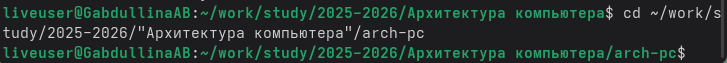
\includegraphics[width=0.9\linewidth,height=\textheight,keepaspectratio]{image/рис12.png}

}

\caption{рис12}

\end{figure}%

\chapter{Выводы}\label{ux432ux44bux432ux43eux434ux44b}

Я освоил процедуру оформления отчетов с помощью легковесного языка
разметки Markdown.

\chapter*{Список
литературы}\label{ux441ux43fux438ux441ux43eux43a-ux43bux438ux442ux435ux440ux430ux442ux443ux440ux44b}
\addcontentsline{toc}{chapter}{Список литературы}

\printbibliography[heading=none]





\end{document}
